\documentclass[12pt, a4paper, oneside]{ctexart}
\usepackage{amsmath, amsthm, amssymb, bm, color, graphicx, geometry, mathrsfs,extarrows, braket, booktabs, array, xcolor, fontspec, appendix, float, subfigure, wrapfig, enumitem}
\usepackage[colorlinks,linkcolor=red,anchorcolor=blue,citecolor=blue,urlcolor=blue,menucolor=black]{hyperref}

%%%% 设置中文字体 %%%%
\setCJKmainfont{方正新书宋_GBK.ttf}[ BoldFont = 方正小标宋_GBK, ItalicFont = 方正楷体_GBK]
%%%% 设置英文字体 %%%%
\setmainfont{Times New Roman}
\setsansfont{Calibri}
\setmonofont{Consolas}

%%%% 设置代码块 %%%%
% 在vscode中使用minted需要先配置python解释器, Ctrl+Shift+P, 输入Python: Select Interpreter选择安装了Pygments的Python版本. 再在setting.json中xelatex和pdflatex的参数中加入 "--shell-escape", 即可
% TeXworks中配置方法参考: https://blog.csdn.net/RobertChenGuangzhi/article/details/108140093
\usepackage{minted}
\renewcommand{\theFancyVerbLine}{
    \sffamily\textcolor[rgb]{0.5,0.5,0.5}{\scriptsize\arabic{FancyVerbLine}}} % 修改代码前序号大小
% 加入不同语言的代码块
\newmintinline{cpp}{fontsize=\small, linenos, breaklines, frame=lines}
\newminted{cpp}{fontsize=\small, linenos, breaklines, frame=lines}
\newmintedfile{cpp}{fontsize=\small, linenos, breaklines, frame=lines}
\newmintinline{matlab}{fontsize=\small, linenos, breaklines, frame=lines}
\newminted{matlab}{fontsize=\small, mathescape, linenos, breaklines, frame=lines}
\newmintedfile{matlab}{fontsize=\small, linenos, breaklines, frame=lines}
\newmintinline{python}{fontsize=\small, linenos, breaklines, frame=lines, python3}  % 使用\pythoninline{代码}
\newminted{python}{fontsize=\small, linenos, breaklines, frame=lines, python3}  % 使用\begin{pythoncode}代码\end{pythoncode}
\newmintedfile{python}{fontsize=\small, linenos, breaklines, frame=lines, python3}  % 使用\pythonfile{代码地址}

%%%% 设置行间距与页边距 %%%%
\linespread{1.2}
\geometry{left=2.5cm, right=2.5cm, top=2.5cm, bottom=2.5cm}

%%%% 定理类环境的定义 %%%%
\newtheorem{example}{例}            % 整体编号
\newtheorem{theorem}{定理}[section] % 定理按section编号
\newtheorem{definition}{定义}
\newtheorem{axiom}{公理}
\newtheorem{property}{性质}
\newtheorem{proposition}{命题}
\newtheorem{lemma}{引理}
\newtheorem{corollary}{推论}
\newtheorem{remark}{注解}
\newtheorem{condition}{条件}
\newtheorem{conclusion}{结论}
\newtheorem{assumption}{假设}
\numberwithin{equation}{section}  % 公式按section编号 (公式右端的小括号)
\newtheorem{algorithm}{算法}

\newsavebox{\nameinfo}
\newenvironment{myTitle}[1]{
    \begin{center}
    {\zihao{-2}\bf #1\\}
    \zihao{-4}\it
}{\end{center}}  % \begin{myTitle}{标题内容}作者信息\end{myTitle}
\newcounter{problem}  % 问题序号计数器
\newenvironment{problem}[1][]{\stepcounter{problem}\par\noindent\textbf{题目\arabic{problem}. #1}}{\smallskip\par}
\newenvironment{solution}[1][]{\par\noindent\textbf{#1解答. }}{\smallskip\par}  % 可带一个参数表示题号\begin{solution}{题号}
\newenvironment{note}{\par\noindent\textbf{注记. }}{\smallskip\par}

%%%% 图片相对路径 %%%%
\graphicspath{{figure/}} % 当前目录下的figure文件夹, {../figure/}则是父目录的figure文件夹
\setlength{\abovecaptionskip}{-0.2cm}  % 缩紧图片标题与图片之间的距离
\setlength{\belowcaptionskip}{0pt} 

%%%% 缩小item,enumerate,description两行间间距 %%%%
\setenumerate[1]{itemsep=0pt,partopsep=0pt,parsep=\parskip,topsep=5pt}
\setitemize[1]{itemsep=0pt,partopsep=0pt,parsep=\parskip,topsep=5pt}
\setdescription{itemsep=0pt,partopsep=0pt,parsep=\parskip,topsep=5pt}

\everymath{\displaystyle} % 默认全部行间公式, 想要变回行内公式使用\textstyle
\DeclareMathOperator*\uplim{\overline{lim}}     % 定义上极限 \uplim_{}
\DeclareMathOperator*\lowlim{\underline{lim}}   % 定义下极限 \lowlim_{}
\DeclareMathOperator*{\argmax}{arg\,max}  % 定义取最大值的参数 \argmax_{}
\DeclareMathOperator*{\argmin}{arg\,min}  % 定义取最小值的参数 \argmin_{}
\let\leq=\leqslant % 简写小于等于\leq (将全部leq变为leqslant)
\let\geq=\geqslant % 简写大于等于\geq (将全部geq变为geqslant)

%%%% 一些宏定义 %%%%
\def\bd{\boldsymbol}        % 加粗(向量) boldsymbol
\def\disp{\displaystyle}    % 使用行间公式 displaystyle(默认)
\def\tsty{\textstyle}       % 使用行内公式 textstyle
\def\sign{\text{sign}}      % sign function
\def\wtd{\widetilde}        % 宽波浪线 widetilde
\def\R{\mathbb{R}}          % Real number
\def\N{\mathbb{N}}          % Natural number
\def\Z{\mathbb{Z}}          % Integer number
\def\Q{\mathbb{Q}}          % Rational number
\def\C{\mathbb{C}}          % Complex number
\def\K{\mathbb{K}}          % Number Field
\def\P{\mathbb{P}}          % Polynomial
\def\N{\mathbb{N}}          % Natural number
\def\Z{\mathbb{Z}}          % Integer number
\def\E{\mathbb{E}}          % Exception
\def\var{\text{Var}}        % Variance
\def\bias{\text{bias}}      % bias
\def\d{\mathrm{d}}          % differential operator
\def\e{\mathrm{e}}          % Euler's number
\def\i{\mathrm{i}}          % imaginary number
\def\re{\mathrm{Re}}        % Real part
\def\im{\mathrm{Im}}        % Imaginary part
\def\res{\mathrm{Res}}      % Residue
\def\L{\mathcal{L}}         % Loss function
\def\O{\mathcal{O}}         % 时间复杂度
\def\wdh{\widehat}          % 宽帽子 widehat
\def\ol{\overline}          % 上横线 overline
\def\ul{\underline}         % 下横线 underline
\def\add{\vspace{1ex}}      % 增加行间距
\def\del{\vspace{-1.5ex}}   % 减少行间距

%%%% 正文开始 %%%%
\begin{document}
\begin{myTitle}{NLP第一次编程作业}
\end{myTitle}
\begin{problem}[(计算最小编辑距离)]
    实现英文最小字符串的编辑距离,计算最小编辑路径并显示结果. 

    \textbf{注:}最小编辑距离定义为:假设s1和s2是两个给定的字符串,考虑对s1字符串进行$n$次\textbf{添加字符、删除字符、替换字符}三种操作,将s1变化为s2,求$n$的最小值.

    \noindent\textbf{例子:}s1 = aadfagha,\ s2 = abcdefgh,则可通过以下5次变换操作将s1变为s2:
    \begin{enumerate}[label=\arabic*)]
        \item 替换:a\textbf{b}dfagha
        \item 添加:ab\textbf{c}dfagha
        \item 添加:abcd\textbf{e}fagha
        \item 删除:abcdefgha
        \item 删除:abcdefgh
    \end{enumerate}
\end{problem}
\begin{solution}
    该问题为经典动态规划(dp)问题,通过设定状态以及状态转移方程即可求解,先进行以下定义:
    \begin{itemize}
        \item 设$s1,s2$为字符串,$l_i$表示字符串$s_i$的长度$(i=1,2)$,$s1[i]$表示字符串$s1$中的第$i$个下标对应的字符.
        \item $s1[i\cdots j]$表示截取字符串$s1$下标从$i$到$j$的子串.
        \item $s1$与$s2$完全匹配,记为$s1=s2$,当且仅当,$s1$与$s2$长度相同,且对任意下标$i$都有$s1[i] == s2[i]$.
    \end{itemize}
    
    设数组$dp[i][j]$为动态规划数组,赋予其中元素以下含义:$dp[i][j]$表示将子串$s1[1\cdots i]$与子串$s2[1\cdots j]$完全匹配所需的最小编辑次数,根据字符串$s1[i]$与$s2[j]$是否相同可分为以下两种情况:
    \begin{enumerate}
        \item 若$s1[i] = s2[j]$,则说明当前字符串末端字符相同,无需编辑修改,于是最小编辑次数直接从$dp[i-1][j-1]$转移得到.
        \item 若$s1[i]\neq s2[j]$,则说明当前字符串末端字符不同,需要通过以上三种修改方式中的一种,使得$s1[1\cdots i]=s2[1\cdots j]$,且编辑次数最小. 于是可从三处得到转移:
        \begin{enumerate}
            \item $dp[i-1][j-1]+1$:表示将$s1[i]$替换为$s2[j]$,则只需保证$s1[1\cdots i-1]=s2[1\cdots j-1]$即可,而使得$s1[1\cdots i-1]=s2[1\cdots j-1]$相同所需的最小步数即为$dp[i-1][j-1]$,再加上当前所需的一步,则是转移方程结果$dp[i-1][j-1]+1$.(剩余两种推导类似)
            \item $dp[i-1][j]+1$:表示将$s1[i]$删除,则只需保证$s1[1\cdots i-1] = s2[1\cdots j]$.
            \item $dp[i][j-1]+1$:表示将$s1[i]$后面添加字符$s2[j]$,则只需保证$s1[1\cdots i] = s2[1\cdots j-1]$.
        \end{enumerate}
    \end{enumerate}
    综上,得到转移方程为
    \begin{equation*}
        dp[i][j] = \begin{cases}
            0,&\quad s1[i] = s2[j],\\
            \min\{dp[i-1][i-1], dp[i-1][j], dp[i][j-1]\}+1,&\quad s1[i]\neq s2[j].
        \end{cases}
    \end{equation*}

    动态规划数组初始条件为$dp[i][0] = dp[0][i] = i,\ (i = 1,2,\cdots, \max\{l_1,l_2\})$,其他值全部初始化为最大值INF,其中$l_i$表示字符串$s_i$的长度.
    
    这样初始化原因是:$dp[i][0]$表示其中一个串的长度为$0$,为使得两个串相同,必定需要删除或添加$i$个字符;其他值初始化为最大值,是因为动态规划是求解最小化问题.

    总时间复杂度:$\O(l_1l_2)$.

    \textbf{动态规划部分代码}:Luogu题目:\href{https://www.luogu.com.cn/problem/P2758}{P2758 编辑距离}
    \begin{cppcode}
#include <iostream>
#include <cstring>
using namespace std;
const int N = 1e4 + 10;  // 字符串最大长度
char s1[N], s2[N];
int dp[N][N];  // dp为动态规划数组
signed main() {
    memset(dp, 127, sizeof(dp));  // 初始化dp数组为极大值
    cin >> s1 >> s2;  // 字符串读入
    int len1 = strlen(s1), len2 = strlen(s2);
    for (int i = 0; i <= max(len1, len2); i++) dp[0][i] = dp[i][0] = i;  // 初始化边界条件
    for (int i = 1; i <= len1; i++) {
        for (int j = 1; j <= len2; j++) {
            if (s1[i-1] == s2[j-1]) {
                dp[i][j] = dp[i-1][j-1];
                continue;
            }
            dp[i][j] = min(dp[i-1][j-1], min(dp[i-1][j], dp[i][j-1])) + 1;
        }
    }
    printf("%d\n", dp[len1][len2]);
    system("pause");
    return 0;
}
    \end{cppcode}

    由于题目还要求输出编辑路径,也就是动态规划每次转移路径,可通过记录每次$dp[i][j]$从哪个位置转移得到的,再从最后一个节点$dp[l_1][l_2]$递归回去,即可得到最优路径上的每次操作,但是这样结果是倒置的,所以需要在回溯过程中进行输出即可. 具体实现请见代码(结果中del表示删除字符,add表示添加字符,chg表示替换字符):

    \begin{cppcode}
#include <iostream>
#include <cstring>
using namespace std;
const int N = 1e4 + 10;  // 字符串最大长度
char s1[N], s2[N];
int dp[N][N], opt[N][N];  // dp为动态规划数组, opt记录每次操作值
// 0: none, 1: delete, 2: add, 3: change
string optName[] = {"none", "del", "add", "chg"}, nowString;
int delta = 0;
void dfs(int i, int j, int o) {
    if (opt[i][j] == 0) dfs(i-1, j-1, 0);
    else if (opt[i][j] == 1) dfs(i-1, j, 1);
    else if (opt[i][j] == 2) dfs(i, j-1, 2);
    else if (opt[i][j] == 3) dfs(i-1, j-1, 3);
    if (o != 0) {
        if (o == 1) nowString.erase(i+delta, 1), delta--;
        else if (o == 2) nowString.insert(i+delta, 1, s2[j]), delta++;
        else nowString[i+delta] = s2[j];
        cout << optName[o] << ": " << nowString << '\n';
    }
}
signed main() {
    memset(dp, 127, sizeof(dp));  // 初始化dp数组为极大值
    memset(opt, -1, sizeof(opt));  // 初始化opt数组为-1
    cin >> s1 >> s2;
    int len1 = strlen(s1), len2 = strlen(s2);
    for (int i = 0; i <= max(len1, len2); i++) dp[0][i] = dp[i][0] = i;
    for (int i = 1; i <= len1; i++) {
        for (int j = 1; j <= len2; j++) {
            if (s1[i-1] == s2[j-1]) {
                opt[i][j] = 0;
                dp[i][j] = dp[i-1][j-1];
                continue;
            }
            int tmp[] = {dp[i-1][j], dp[i][j-1], dp[i-1][j-1]}, mn = 1e9, mnId;  // mn记录当前最小值,mnId记录从哪个位置转移得到的
            for (int k = 0; k < 3; k++) {
                if (tmp[k] < mn) {
                    mn = tmp[k];
                    mnId = k;
                }
            }
            dp[i][j] = mn + 1;
            opt[i][j] = mnId + 1;
        }
    }
    printf("minimal step: %d\n", dp[len1][len2]);
    //---------- 以上部分为动态规划部分 ----------
    nowString = string(s1);
    cout << "s1:  " << nowString << '\n';
    dfs(len1, len2, 0);
    system("pause");
    return 0;
}

#if 0
Input:
aadfagha
abcdefgh

Output:
minimal step: 5
s1:  aadfagha
chg: abdfagha
add: abcdfagha
add: abcdefagha
del: abcdefgha
del: abcdefgh
#endif
    \end{cppcode}
\end{solution}

\begin{problem}{(修改操作代价改变最小编辑距离)}
    记删除,添加,替换的权重分别为$w_1,w_2,w_3$,于是只需要将初始化部分和$dp$数组转移处的权重进行调整即可:
    \begin{itemize}
        \item 初始化部分:$dp[i][0] = w_1\cdot i$表示需要删除掉$s1$中$i$个字符,则权重为$w_1\cdot i$,类似的,$dp[0][j] = w_2\cdot j$,表示需要添加$j$个字符.
        \item 转移方程
        \begin{equation*}
            dp[i][j]=\begin{cases}
                0,&\quad s1[i]=s2[j],\\
                \min\left\{\begin{aligned}
                    &dp[i-1][j]+w_1,\\
                    &dp[i][j-1]+w_2,\\
                    &dp[i-1][j-1]+w_3
                \end{aligned}\right\},&\quad s1[i]\neq s2[j].
            \end{cases}
        \end{equation*}
    \end{itemize}
    仅在上一题代码上稍加修改即可,下面仅列出修改的重要部分.
    \begin{cppcode}
...
int w[3];  // w[3]分别对应删除,添加,替换的权重
...
signed main() {
...
    cin >> w[0] >> w[1] >> w[2];  // 读入权重
...
    for (int i = 0; i <= max(len1, len2); i++) dp[0][i] = i * w[1], dp[i][0] = i * w[0];  // 带权重的初始化
    for (int i = 1; i <= len1; i++) {
        for (int j = 1; j <= len2; j++) {
            ...
            for (int k = 0; k < 3; k++) {
                if (tmp[k] < mn) {
                    mn = tmp[k] + w[k];  // 对第k个操作加上权重
                    mnId = k;
                }
            }
            dp[i][j] = mn;
            opt[i][j] = mnId + 1;
        }
    }
    printf("minimal weight: %d\n", dp[len1][len2]);
    //---------- 以上部分为动态规划部分 ----------
    ...  //  递归部分完全一致
    return 0;
}

#if 0
Input:
aadfagha
abcdefgh
1 2 1

Output:
minimal weight: 6
s1:  aadfagha
add: abadfagha
chg: abcdfagha
chg: abcdeagha
chg: abcdefgha
del: abcdefgh
#endif
    \end{cppcode}
    可以看到,提高了加入字符操作所具有的权重,最优路径从原来两次添加降为一次添加,并增加两次替换操作.
\end{problem}

\textbf{源代码:}
\begin{enumerate}
    \item 纯动态规划解决问题:\texttt{calc\_distance\_dp.cpp}
    \item 显示编辑路径:\texttt{calc\_distance\_complete.cpp}
    \item 带权重且显示编辑路径:\texttt{calc\_distance\_complete\_weight.cpp}
\end{enumerate}

\end{document}

\iffalse
%%%% 表格模板 %%%%
\renewcommand\arraystretch{0.8} % 设置表格高度为原来的0.8倍
\begin{table}[!htbp] % table标准
    \centering % 表格居中
    \begin{tabular}{p{1cm}<{\centering}p{1cm}<{\centering}p{3cm}<{\centering}p{5cm}<{\centering}} % 设置表格宽度
    %\begin{tabular}{cccc}
        \toprule
        $x_i$ & $f[x_1]$ & $f[x_i, x_{i+1}]$ & $f[x_i, x_{i+1}, x_{i+2}]$ \\
        \midrule
        $x_0$ & $f(x_0)$ &                  &                          \\
        $x_0$ & $f(x_0)$ & $f'(x_0)$        &                          \\
        $x_0$ & $f(x_1)$ & $\frac{f(x_1)-f(x_0)}{x_1-x_0}$ & $\frac{f(x_1)-f(x_0)}{(x_1-x_0)^2}-\frac{f'(x_0)}{x_1-x_0}$\\
        \bottomrule
    \end{tabular}
\end{table}

%%%% 文字环绕图片, 标题加注释 %%%%
{ % 一般将文字环绕部分的图和文字, 用大括号括起来, 避免对文字外的格式发生影响
\begin{wrapfigure}[13]{r}{.5\linewidth} % 文字环绕行数为13行, 图片靠右 (l为靠左), 图片占0.5的行宽
    \centerin右
    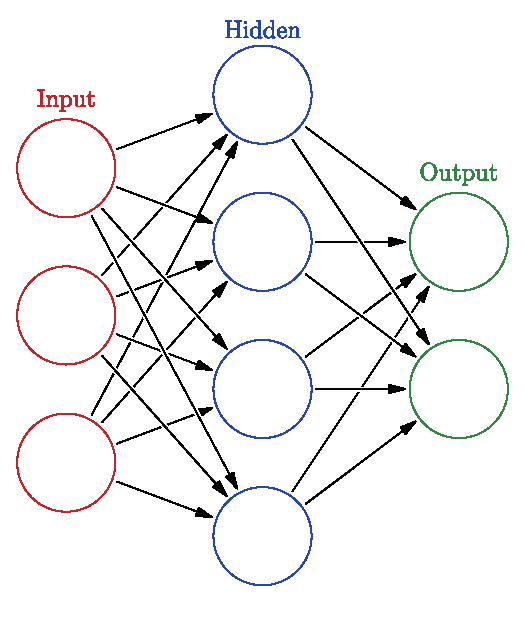
\includegraphics[scale=0.7]{neural_network.eps} % scale=0.7按比例缩放70%
    \caption{神经网络结构\protect\footnotemark[1]} % 记得加\protect, 设置1号脚标
    \label{figure-神经网络结构}
\end{wrapfigure}
\footnotetext[1]{图片来源: \url{https://en.wikipedia.org/wiki/File:Colored_neural_network.svg}}
文字文字
}

%%%% 普通图片, 标题加注释 %%%%
\begin{figure}[htbp] % h: 当前位置, t: 顶部, b: 底部, p: 浮动页, 这样组合指的是使用这个顺序进行排版
    \centering
    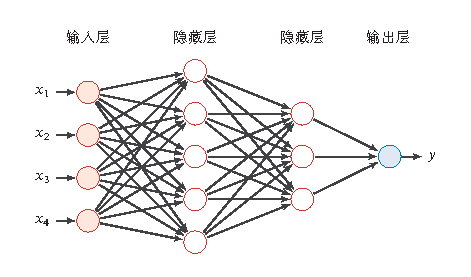
\includegraphics[scale=0.5]{前馈神经网络.eps}
    \caption{前馈神经网络\protect\footnotemark[1]}
    \label{figue-前馈神经网络}
\end{figure}
\footnotetext[1]{图片来源: 邱锡鹏, 神经网络与深度学习 \cite{ref-qxp}, 第92页}

%%%% 多组图 %%%%
    \begin{figure}[htbp]
        \centering
        \subfigure[迭代1次]  % 子图的标题
        {
            % 如果一行放三个图改成0.3\linewidth即可
            \begin{minipage}[b]{.45\linewidth}  % 0.45排版行距, 即一行放2个图, 一行放不下就换行
                \centering
                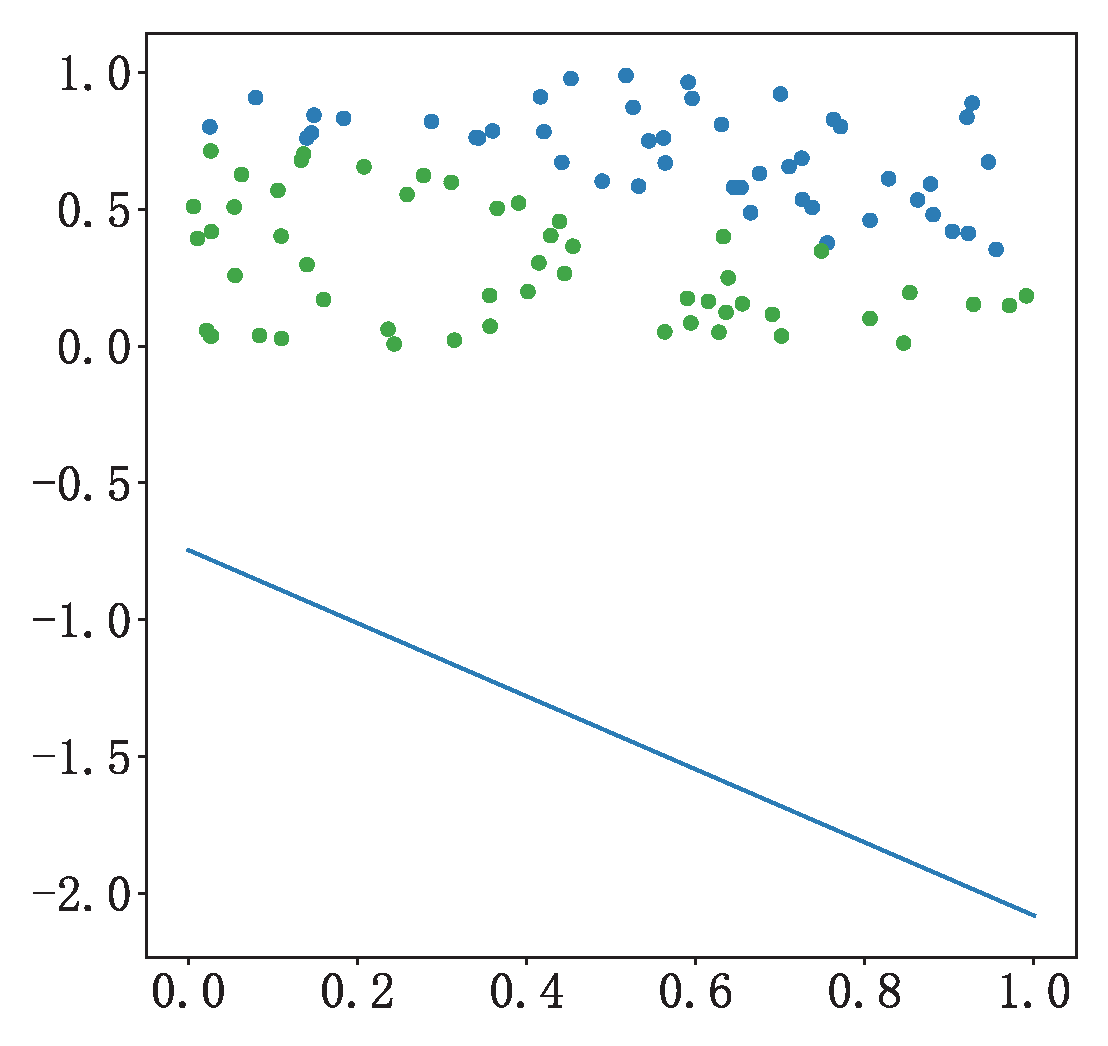
\includegraphics[scale=0.35]{1.eps}
            \end{minipage}
        }
        \subfigure[迭代100次]
        {
            \begin{minipage}[b]{.45\linewidth}
                \centering
                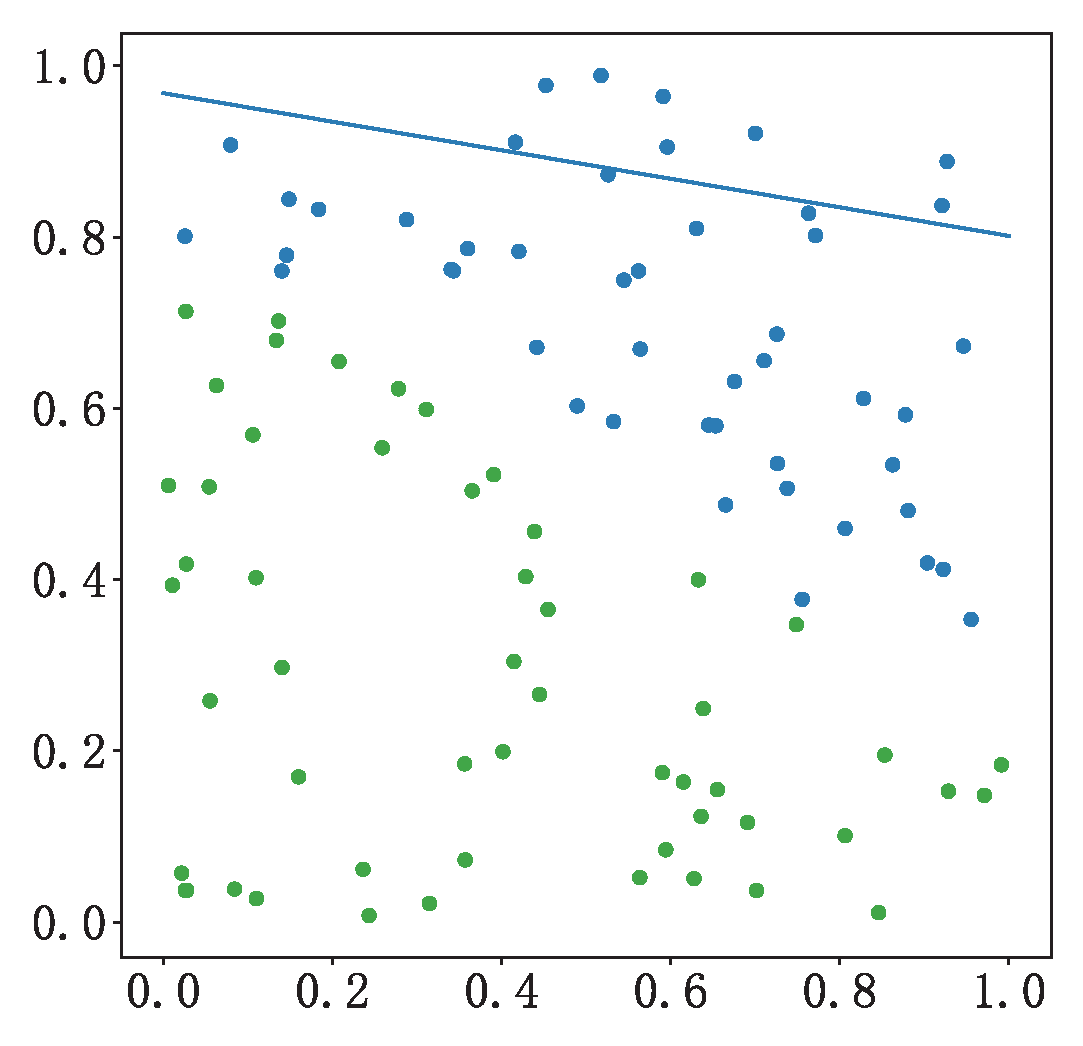
\includegraphics[scale=0.35]{100.eps}
            \end{minipage}
        }
        \subfigure[迭代500次]
        {
            \begin{minipage}[b]{.45\linewidth}
                \centering
                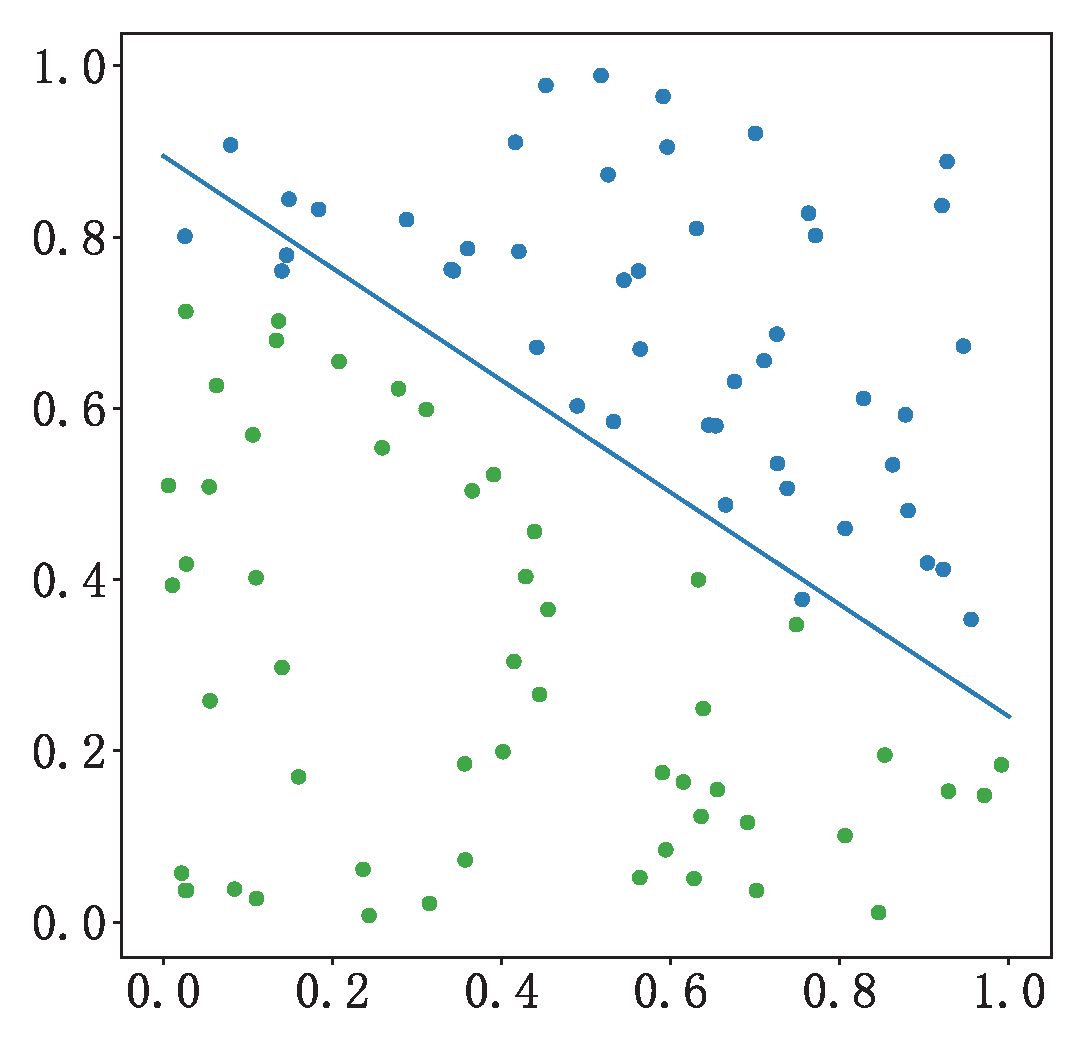
\includegraphics[scale=0.35]{500.eps}
            \end{minipage}
        }
        \subfigure[迭代2000次]
        {
            \begin{minipage}[b]{.45\linewidth}
                \centering
                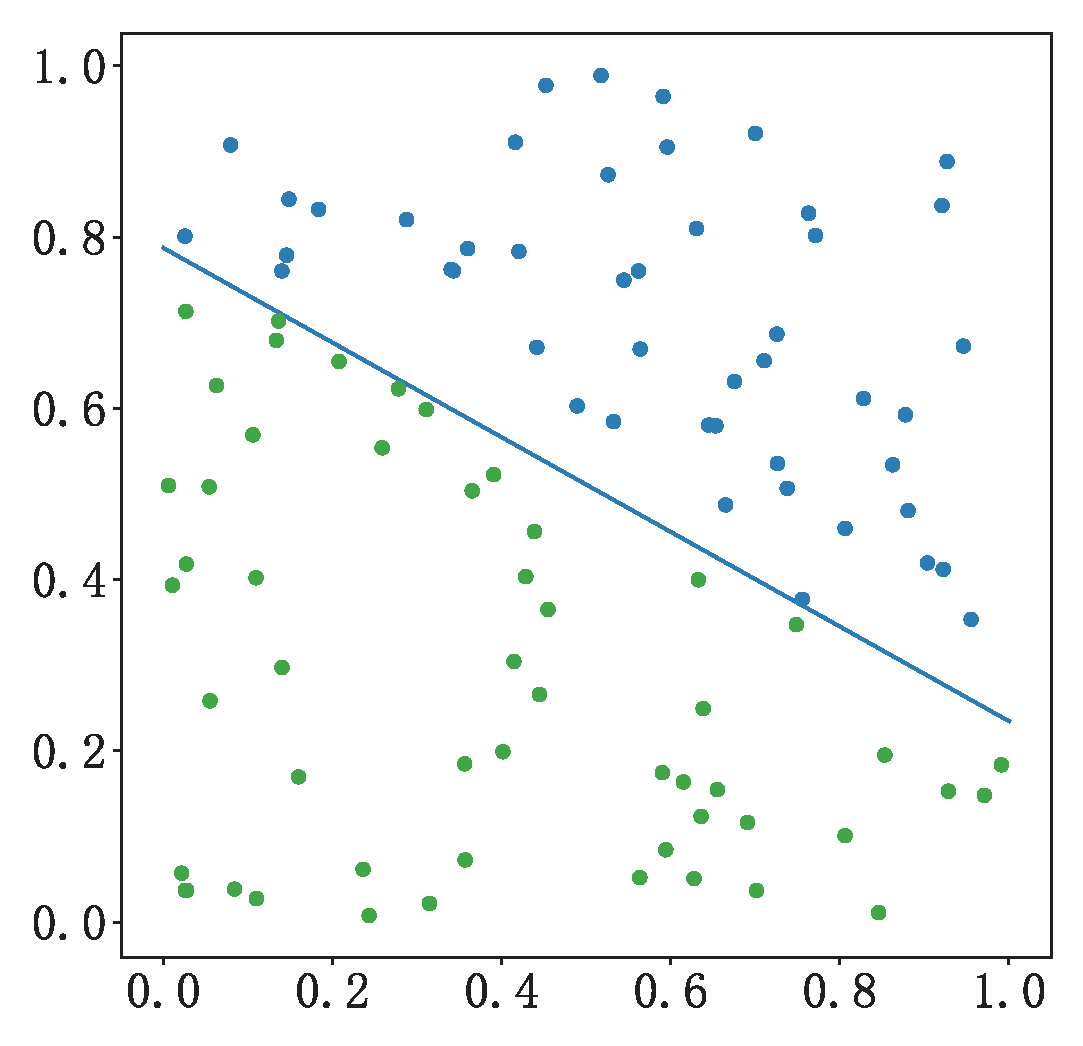
\includegraphics[scale=0.35]{2000.eps}
            \end{minipage}
        }
        \caption{迭代过程图}
        \label{figure-迭代过程图}
    \end{figure}
\fi
